\documentclass[tesis]{tesis-usach}

%\usepackage[linesnumbered, ruled, vlined, boxed, commentsnumbered, spanish]{algorithm2e}
%\usepackage{algpseudocode}

\usepackage{import}
%\usetikzlibrary{arrows, calc, decorations.markings, math}
%\usetikzlibrary{matrix, chains, positioning, decorations.pathreplacing, shapes, snakes}

% https://tex.stackexchange.com/questions/129677/automatic-capitalization-of-sectioning-headings
\makeatletter
%\def\@makechapterhead#1{
%	\begingroup
%		\Large\bfseries\MakeUppercase{\@chapapp{} \thechapter. #1}
%		\vspace{20pt}
%	\endgroup
%}

%\renewcommand{\section}{
%	\@startsection{section}{1}{\z@}
%	{2pt}%{6.5ex plus 1ex minus .2ex}
%	{0.5cm}%{2.3ex plus .2ex}
%	{\large\bfseries\MakeUppercase}%*[<altheading>]{<heading>}
%}

%%\titleformat{\chapter}{\bfseries\Large\vspace*{-4.0cm}}{\filright\Large\MakeUppercase\chaptertitlename\ \thechapter.\ }{0pt}{\filright\MakeUppercase}[\vspace{1.5pt}]
%%\titlespacing*{\chapter} {0pt}{85pt}{20pt}
%
%\renewcommand{\section}{
%	\@startsection{section}{1}{\z@}
%	{2pt}%{6.5ex plus 1ex minus .2ex}
%	{0.5cm}%{2.3ex plus .2ex}
%	{\large\bfseries\MakeUppercase}%*[<altheading>]{<heading>}
%}
%%\titleformat{\section}{\bfseries\large\vspace{2pt}}{\large\MakeUppercase\thesection\ \vspace{2pt} }{0pt}{\MakeUppercase}[\vspace*{0.5cm}]
%%\titlespacing*{\section} {0pt}{6.5ex plus 1ex minus .2ex}{2.3ex plus .2ex}
%
%\renewcommand{\subsection}{\@startsection{subsection}{2}{\z@}%
%             {-3.25ex\@plus -1ex \@minus -.2ex}%
%             {1.5ex \@plus .2ex}%
%             {\normalfont\large\scshape\bfseries}}
%						 %\titleformat{\subsection}{\bfseries\normalsize\vspace{2pt}}{\normalsize\thesubsection\ }{0pt}{\vspace*{0.5cm}}
%						 %\titlespacing*{\subsection} {0pt}{6.5ex plus 1ex minus .2ex}{2.3ex plus .2ex}
%
%\renewcommand{\subsubsection}{\@startsection{subsubsection}{2}{\z@}%
%             {-3.25ex\@plus -1ex \@minus -.2ex}%
%             {1.5ex \@plus .2ex}%
%             {\normalfont\normalsize\scshape\bfseries}}
%						 %\titleformat{\subsubsection}{\itshape\normalsize\vspace{1.0cm}}{\itshape\thesubsubsection\ }{0pt}{\vspace*{0.5cm}\itshape}
%						 %\titlespacing*{\subsubsection}{0pt}{3.25ex plus 1ex minus .2ex}{1.5ex plus .2ex}
\makeatother


\title{Análisis de la eficiencia del entrenamiento de redes neuronales profundas basado en simulated annealing}
\informe{Informe}
\facultad{Facultad de Ingenieria}
\departamento{Departamento de ingenieria informática}

\author{Felipe Alberto Reyes González}
\programa{Magíster en Ingeniería Informática}
\profesor{Victor Parada}
\celular{890 26 317}
\correo{felipe.reyesg@usach.cl}
\date{\today}

\let\cite\shortcite
\usepackage{layouts}

\begin{document}
\printinunitsof{cm}{\pagevalues}

\pagediagram
	\renewcommand{\BOthers}[1]{et al.\hbox{}}%
	\maketitle
	\makecopyright
	\frontmatter
	\indice
	\mainmatter

	%%%%%%%%%%%%%%%%%%%%%%%%%%%%
	% Inicio contenido
	%%%%%%%%%%%%%%%%%%%%%%%%%%%%
	\chapter{Introducción}
\section{Antecedentes y motivación}
%[Bishop] Neural Network for pattern recognition :: 77 y 116
Las redes neuronales ({\em Neural Networks}, NN) son sistemas de procesamiento de información que basan su estructura en una analogía de las redes neuronales biológicas. Consisten en un conjunto de elementos de procesamiento simple llamados nodos, estos nodos están dispuestos en una estructura jerarquica y conectadas entre si por un valor numérico llamado peso que, mediante un proceso de entrenamiento, varia su valor.

La actividad que una neurona realiza en una NN es simple. El proceso consiste en ponderar las entradas de la neurona por los pesos de las conexiones de la neurona para luego ser sumadas y entregadas a la función de activación asociada a la neurona \cite{McCulloch1943}. La salida corresponderá a la respuesta que la neurona genera a la entrada que se presentada.

Las neuronas con una función de activación umbral, fueron estudiadas por \citeA{Rosenblatt1962} quién las denominó {\em perceptrón}. El modelo básico se compone de 3 capas conectadas consecutivamente. La primera capa corresponde a la capa de entrada, que recibe el patrón de entrada a clasificar. La segunda capa contiene las neuronas de asociación o detección de características. Y la tercera capa es la capa de salida, que contiene las neuronas que reconocen los patrones. La limitación de los perceptrones se debe a capacidad de clasificación basado en el umbral, lo que no permite clasificar patrones mas complejos.

El conjunto de $n$ neuronas se llamará capa, y una NN puede estar compuesta de una o más capas. Cada capa estará compuesta por una cantidad de neuronas que no necesariamente será la misma para todas las capas, y estarán dispuesta en forma consecutiva de tal manera que las capas se conecten unas con otras y siempre hacia adelante. La primera capa, la de entrada, recibirá un patrón que será entregado a las distintas neuronas que la capa posea. Cada neurona de la capa de entrada procesará los datos y generará una salida que servirá de entrada para la capa siguiente, repitiendo el proceso para cada una de las capas de la NN hasta llegar a la capa de salida, en cuyo caso la salida representará la respuesta de la red, concretando así el ciclo.

% https://www.neuraldesigner.com/blog/5_algorithms_to_train_a_neural_network
Las NN han sido utilizadas para la clasificación de entradas, y han sido diseñados diversos métodos para entrenar la red y que los pesos se adapten de tal manera que la salida de la red sea representativa de la salida esperada, a esto método de entrenamiento se le llama supervisado. Dentro de los métodos de entrenamiento existentes se encuentra el método del gradiente descendente, el método de Newton, el gradiente conjugado, el método quasi-Newton, o el algoritmo Levenberg-Marquardt. El más utilizado es el método del gradiente, que consiste en actualizar los pesos de las distintas neuronas en función de la dirección contraría al gradiente de la función de activación, logrando minimizar el error.

El gradiente descendente es el mas simple de los métodos. Este requiere información del gradiente del vector, por lo tanto corresponde a un método de primer orden. El método comienza en un punto inicial y, mientras el criterio de parada no se cumpla, la solución inicial se moverá en la dirección contraria al gradiente a razón de una taza de aprendizaje establecida. La taza de aprendizaje es quién decide cuan largo será el paso, si éste es muy grande, puede que la convergencia a la solución sea superada por un paso muy grande, en cambio, una taza de aprendizaje my pequeña puede demorar la convergencia.

El método de Newton es un método de segundo orden, pues hace uso de la matriz Hessiana. El objetivo de este método es encontrar una mejor dirección de entrenamiento mediante el uso de la segunda derivada de la función de perdida. Considera una aproximación cuadrática de la función en la solución inicial utilizando una expansión de la serie de Taylor. De esta manera, el método de Newton permite mover la solución inicial en función de la inversa de la matriz Hessiana, que pasará a ser la dirección de entrenamiento de Newton.

%El método del gradiente conjugado, fue propuesto por Fletcher and Reeves (1964), es un punto intermedio entre el gradiente descendente y el método de Newton. Utiliza sucesivas direcciones
El método del gradiente del conjugado fue propuesto por \citeA{Fletcher1964}, utiliza sucesivas direcciones conjugadas basadas en el gradiente y el residuo. Si la función objetivo es cuadrática y la dirección de búsqueda es minimizada exactamente en cada iteración, el método converge de forma cuadrática. \citeA{Leonard1990} han utilizado el método para entrenar redes neuronales como alternativa a la retropropagación. Los pesos de una red se actualizan de acuerdo con una búsqueda unidencial en la dirección de descenso $S(n)$ de la siguiente forma:
\begin{eqnarray}
	\Delta W(n) = \lambda(n)S(n)
\end{eqnarray}

Y la dirección de descenso $S(n)$ se calcula a partir del gradiente de iteraciones pasadas y presentes como muestra la ecuación \ref{eq:s(n)}
\begin{eqnarray}
	S(n) &=& G(n) + \frac{||G(n)||}{||G(n - 1)||}S((n - 1))\label{eq:s(n)}
\end{eqnarray}

Para que las direcciones de descenso permanezcan conjugadas, la búsqueda unidirecional, en cada iteración, tiene que ser llevada con alta precisión. Sin embargo, después de muchas iteraciones, las direcciones podrían llegar a ser casi paralelas. Para superar esta dificultad, \citeA{Fletcher1964} sugieren volver a iniciar el procedimiento igualando la dirección de descenso al gradiente en cada iteración $(t + 1)$, donde $(t)$ es el número total de pesos en la red.
%\paragraph{Aprendizaje por corrección del error}: La salida de la NN se compara con la salida esperada, y la diferencia entre ambos valores se utiliza para corregir los pesos de las neuronas. Los pesos de las neuronas se ajustan en función de dicho error hasta ajustarse a los datos que se utilizan para el entrenamiento.

%\paragraph{Aprendizaje estocástico}: Consiste en modificar aleatoriamente los valores de los pesos y observar los resultados para evaluarlos respecto de la salida deseada. Las redes que utilizan este tipo de aprendizaje son una analogía de algún proceso físico basado en estados de energía, donde la red sería el grado de estabilidad y se buscaría el estado de mínima energía, que es el estado donde la respuesta de la red se ajusta de mejor manera a los datos. [37]

\section{Descripción del problema}
%\subsection{El desvanecimiento del gradiente}
La retropropagación basa su funcionamiento en la regla de la cadena para poder calcular los gradientes, y a medida que el error se propaga hacia la capa de entrada de la red él gradiente comienza a disminuír su valor por cada capa que atraviesa. Esto significa que el gradiente disminuirá de manera exponencial, lo que representa un problema para una red de muchas capas, ya que las capas mas cercanas a la capa de entrada necesitarán más tiempo para ser entrenadas.

\section{Solución propuesta}
\subsection{Características de la solución}
Mediante el uso de el algoritmo {\em simulated annealing} se busca analizar la eficiencia que la NN alcanza en una red neuronal profunda frente a otros métodos de aprendizaje.

\subsection{Propósito de la solución}
El propósito de la solución es aportar en el campo de las redes neuronales y la clasificación de datos, proporcionando un análisis comparativo de la convergencia de distintas redes.
\section{Objetivos y alcances del proyecto}
\subsection{Objetivo general}
Evaluar el desempeño del algoritmo {\em simulated annealing} y su efecto sobre entrenamiento de redes neuronales profundas.

\subsection{Objetivos específicos}
Los objetivos establecidos para el presente trabajo son descritos a continuación
\begin{enumerate}
    \item Definir las reglas de aprendizaje a implementar.
    \item Construir los conjuntos de datos de entrada y salida a analizar.
	\item Establecer los parámetros de las redes neuronales para la experimentación.
	\item Entrenar las redes con los distintos conjuntos de datos.
    \item Establecer las conclusiones del trabajo.
\end{enumerate}

\subsection{Alcances}

\section{Metodología y herramientas utilizadas}
\subsection{Metodología de trabajo}
Considerando el aspecto investigativo del trabajo, se considera la utilización del método científico. Entre las actividades que componen la metodología, \citeA{Sampieri2006} describe los siguientes pasos para desarrollar una investigación:

\begin{itemize}
	\item Formulación de la hipótesis: Las redes neuronales que adolecen del desvanecimiento del gradiente se ven beneficiadas por el uso del algoritmo {\em simulated annealing} en la convergencia.

	\item Marco teórico: Una revisión de la literatura donde se aborda el problema planteado, para situarse en el contexto actual de los problemas. Se describirán redes neuronales que buscan solucionar el mismo problema.

	\item Diseño de la solución: Se deberá diseñar el experimento para generar los datos que permitan sustentar las comparaciones entre las distintas redes. Diseñar y ejecutar el experimento basado en entradas equivalentes.

	\item Análisis y verificación de los resultados: Los resultados se analizarán considerando los valores de convergencia de los distintos métodos.

	\item Presentación de los resultados: Se presentarán tablas que describan los resultados obtenidos y que se consideren pertinentes.

	\item Conclusiones obtenidas en el desarrollo de la investigación.
\end{itemize}

\subsection{Herramientas de desarrollo}
Para el desarrollo y ejecución de los experimentos se utilizará un equipo con las siguientes características
\begin{table}[H]
	\centering
	\begin{tabular}{|l|l|}\hline
        Sistema Operativo	& Solus 2017.04.18.0 64-bit\\\hline
        Procesador				 & Intel$^\circledR$ Core\texttrademark i5-2450M CPU @ 2.50GHz x 4\\\hline
        RAM							  & 7.7Gb\\\hline
		Gráficos					& Intel$^\circledR$ Sandybridge Mobile\\\hline
		Almacenamiento	   & 935.6 GB\\\hline
	\end{tabular}
	\caption{Especificaciones del equipo}
\end{table}

El software que se utilizará es:
\begin{itemize}
	\item Plataforma de desarrollo: Atom.
	\item Lenguaje de programación: Python.
	\item Sistema de redes neuronales: Keras API \cite{Keras2015}.
	\item Herramienta ofimática: \LaTeX.
\end{itemize}

	\chapter{Aspectos teóricos y revisión de la literatura}
\section{Aspectos teóricos}
\subsection{Algoritmo de retropropagación}
El elemento básico de las redes neuronales ({\em Neural Networks}, NN) es el nodo, que recibe un vector de entrada para producir una salida. Cada entrada tiene asociado un vector de pesos $w$, que se va modificando durante el proceso de aprendizaje. Cada unidad aplica una función $f$ sobre la suma ponderada de las entradas ponderada
%\begin{eqnarray}
%	$$ y_{i} = \sum_{j} w_{ij}y_{j}\label{eq:entrada} $$
%\end{eqnarray}
donde el resultado puede servir como entrada de otras unidades.

Existen dos fases importante dentro del modelo
\begin{itemize}
	\item Fase de entrenamiento: Se usa un conjunto de datos o patrones de entrenamiento para determinar los pesos que definen el modelo de la NN. Se calculan de manera iterativa, de acuerdo con los valores de entrenamiento, con el objeto de minimizar el error cometido entre la salida obtenida por la NN y la salida deseada.

	\item Fase de prueba: Durante el entrenamiento, el modelo se ajusta al conjunto de entrenamiento, perdiendo la habilidad de generalizar su aprendizaje a casos nuevos, a esta situación se le llama sobreajuste.
	Para evitar el sobreajuste, se utiliza un segundo grupo de datos diferentes, el conjunto de validación, que permitirá controlar el proceso de aprendizaje.
\end{itemize}
Los pesos óptimos se obtienen minimizando una función. Uno de los criterios utilizados es la minimización del error cuadrático medio entre el valor de salida y el valor real esperado.


\subsection{El perceptrón multicapa}
Dentro de las redes neuronales, el perceptrón multicapa es una de las arquitecturas más usadas para resolver problemas. Esto es debido a que poseen la capacidad de ser un aproximador universal \cite{Minsky1969b}. Esto no implica que sea una de las redes más potentes o con mejores resultados, el perceptrón multicapa posee una serie de limitaciones, como el proceso de aprendizaje para problemas que dependan de un gran número de variables, la dificultad para realizar un análisis teórico de la red debido a la presencia de componentes no lineales y a la alta conectividad.

\subsubsection{Arquitectura}
El perceptron multicapa posee una estructura de capas compuestas por neuronas. Cada una de las capas está formada por un conjunto de neuronas y se distinguen tres tipos de capas: la capa de entrada, las capas ocultas y la capa de salida.

\begin{imagen}
	\scalebox{0.8}{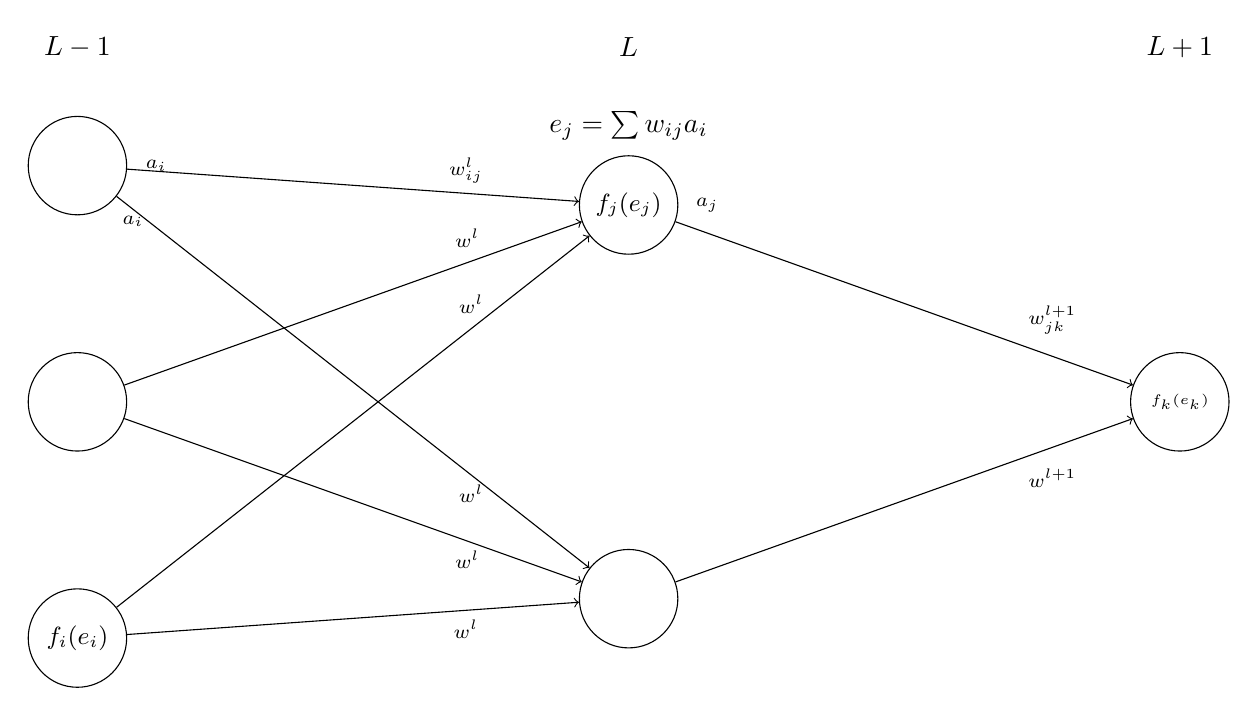
\begin{tikzpicture}

	\tikzstyle{nodo}=[circle, draw, minimum size=1.25cm]
	\tikzstyle{upw}=[dashed, red, ->, line width = 1pt]

	\coordinate (l_0) at (0, 4.5);
	\coordinate (l_1) at (7, 4.5);
	\coordinate (l_2) at (14, 4.5);

	\coordinate (f_1_1) at (0, 3); % CAPA ENTRADA
	\coordinate (f_1_2) at (0, 0); % CAPA ENTRADA
	\coordinate (f_1_3) at (0, -3); % CAPA ENTRADA
	\coordinate (f_2_1) at (7, 2.5); % CAPA OCULTA 1
	\coordinate (f_2_2) at (7, -2.5); % CAPA OCULTA 1
	\coordinate (f_3_1) at (14, 0); % CAPA SALIDA

	\node[] (l_0) at (l_0) {$L - 1$};
	\node[] (l_1) at (l_1) {$L$};
	\node[] (l_2) at (l_2) {$L + 1$};

	\node[nodo] (f_1_1) at (f_1_1) {}; % CAPA ENTRADA
	\node[nodo] (f_1_2) at (f_1_2) {}; % CAPA ENTRADA
	\node[nodo] (f_1_3) at (f_1_3) {\small $f_i(e_i)$}; % CAPA ENTRADA
	\node[nodo] (f_2_1) at (f_2_1) {\small $f_j(e_j)$}; % CAPA OCULTA 1
	\node[nodo] (f_2_2) at (f_2_2) {}; % CAPA OCULTA 1
	\node[nodo] (f_3_1) at (f_3_1) {\tiny $f_k(e_k)$}; % CAPA SALIDA


	\draw[->, font=\scriptsize] (f_1_1) node[right of=f_1_1] {$a_{i}$} -- node[pos=0.75, above] (w_1_1) {$w^{l}_{ij}$} (f_2_1);
	\draw[->, font=\scriptsize] (f_1_2) node[below right of=f_1_1] {$a_{i}$} -- node[pos=0.75, above] (w_1_2) {$w^{l}_{}$} (f_2_1);
	\draw[->, font=\scriptsize] (f_1_3) -- node[pos=0.75, above] (w_1_3) {\scriptsize$w^{l}_{}$} (f_2_1);
	\draw[->, font=\scriptsize] (f_1_1) -- node[pos=0.75, below] (w_2_1) {$w^{l}_{}$} (f_2_2);
	\draw[->, font=\scriptsize] (f_1_2) -- node[pos=0.75, below] (w_2_2) {$w^{l}_{}$} (f_2_2);
	\draw[->, font=\scriptsize] (f_1_3) -- node[pos=0.75, below] (w_2_3) {$w^{l}_{}$} (f_2_2);

	\node[above of=f_2_1] {$e_{j} = \sum w_{ij}a_i$};

	\draw[->, font=\scriptsize] (f_2_1) node[right of=f_2_1] {$a_{j}$} -- node[pos=0.75, above right] (w_j_k) {$w^{l+1}_{jk}$} (f_3_1);
	\draw[->, font=\scriptsize] (f_2_2) -- node[pos=0.75, below right] {$w^{l+1}$} (f_3_1);


	%\draw[upw] (f_3_1) to[bend left=20] (w_1_1);
	%\draw[upw] (f_3_1) to[bend left=20] (w_1_2);
	%\draw[upw] (f_3_1) to[bend left=20] node[pos=0.7, right] {$w^{l}_{ij} - \alpha\frac{\partial e}{\partial w}$} (w_1_3);


	%\draw[upw] (f_4_1) to[bend right=20] node[pos=0.8, right] {$w^{l+1}_{jk} - \alpha\frac{\partial e}{\partial w^{l+1}_{jk}}$} (w_j_k);

	%\node[above right of=w_j_k, node distance=3cm] {$\frac{\partial e}{\partial w^{l+1}_{jk}}=-(s_i - y_i)\frac{\partial y_i}{\partial w^{l+1}_{jk}}$};
\end{tikzpicture}
}
	\caption{Perceptrón multicapa}
	\label{fig:neurona}
\end{imagen}

En la figura \ref{fig:neurona} se observa que las conexiones van siempre hacia adelante. Las neuronas de la capa $l$ se conectan con las neuronas de la capa $l + 1$. Las neuronas de la capa de entrada se encargan de recibir los patrónes y propagar dichas señales a las neuronas de la capa siguiente. La última capa, la capa de salida, proporciona la respuesta de la red al patrón presentado. Las neuronas de las capas ocultas realizan el procesado de las señales generadas por el patrón de entrada.

\subsubsection{Propagación de la entrada y el algoritmo de retropropagación}
El perceptrón multicapa define una relación entre la entrada y la salida. Esta relación se obtiene propagando hacia adelante los valores de las variables de entrada, es por esto que también se les llama redes {\em feedforward}. Cada neurona de la red procesa la entrada recibida y produce una respuesta que se propaga, mediante las conexiones, hacia las neuronas de la capa siguiente.

Si un perceptrón multicapa con $C$ capas y $n_c$ neuronas en la capa $c$, donde $W_c = (w^{c}_{ij})$ es la matriz de pesos, $w^{c}_{ij}$ representará el peso de la conexion de la neurona $i$ de la capa $c$ hasta la neurona $j$ de la capa siguiente. Denotaremos $a^{c}_{i}$ a la activación de la neurona $i$ de la capa $c$ que se calcula de la siguiente manera:
\begin{itemize}
	\item {\bf Activación de una neurona de la capa de entrada}: Las neuronas se encargan de transmitir la entrada recibida, por lo tanto $$ a^{1}_{i} = x_{i}, i = 1, 2, \cdots, n$$ donde $X = (x_1, x_2, \cdots, x_n)$ representa el vector de entrada.

	\item {\bf Activación de una neurona de la capa oculta}: Las neuronas de una capa oculta procesa la información recibida aplicando la función de activación $f$ a la suma de los productos de la entrada por sus pesos, es decir $$ a^{c}_{i} = f\left(\sum^{n_{c - 1}}_{j=1} w^{c - 1}_{ji}a^{c - 1}_{j} + \theta^{c}_{i}\right), i = 1, 2, \cdots, n_c; c = 2, 3, \cdots, C - 1$$ donde $a^{c - 1}_{j}$ es la salida de la capa anterior a $c$.

	\item {\bf Activación de una neurona de la capa de salida}: La activación de una neurona de la capa de salida viene dada por la función de activación $f$ aplicada a la suma de los productos de la entrada por sus pesos, es decir $$ y_{i} = a^{c}_{i} = f\left(\sum^{n_{c - 1}}_{j=1} w^{C - 1}_{ji}a^{C - 1}_{j} + \theta^{C}_{i}\right), i = 1, \cdots, n_c$$ donde $Y = (y_1, y_2, \cdots, y_{n_{c}})$ es el vector de salida.
\end{itemize}

La función $f$ es la función de activación de la neurona. Las funciones de activación mas utilizadas son la sigmoidal y la tangente hiperbólica, descritas en las escuaciones \ref{eq:sigm} y \ref{eq:tanh} respectivamente.
\begin{eqnarray}
	f_{sigm}(x) &=& \frac{1}{1+\exp(-x)}\label{eq:sigm}\\
	f_{tanh}(x) &=& \frac{1 - \exp(-x)}{1 + \exp(-x)}\label{eq:tanh}
\end{eqnarray}

Ambas funciones poseen como imagen intervalo de valores entre $[0, 1]$ y $[-1, 1]$ como se observa en la figura \ref{fig:funciones}.% y están descritas por las ecuaciones \ref{eq:sigm} y \ref{eq:tanh}.

\begin{imagen}
	\scalebox{1.0}{
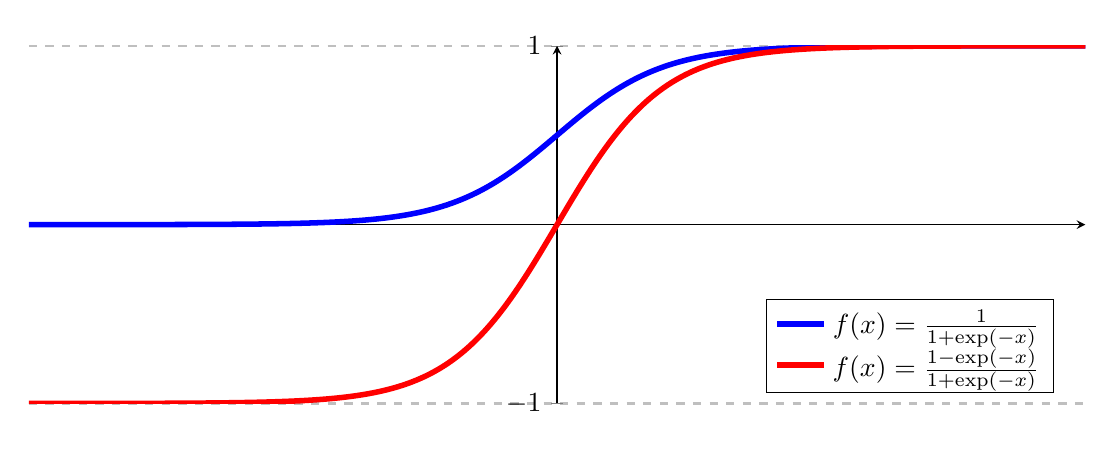
\begin{tikzpicture}
\begin{axis}[ymin=-1, ymax = 1, axis lines = left, legend pos=south east, width=15cm, xmajorticks=false, ytick={-1, +1}, axis lines=middle, y post scale=0.4, ymajorgrids=true, major grid style={dashed, line width=0.8pt}, yticklabel pos=left]
%Here the blue parabloa is defined
\addplot[domain=-10:10, samples=1000, color=blue, line width=2pt]{1/(1 + exp(-x))};
\addplot[domain=-10:10, samples=1000, color=red, line width=2pt]{(1 - e^(-x))/(1 + e^(-x))};
\addlegendentry{$f(x) = \frac{1}{1+\exp(-x)}$}
\addlegendentry{$f(x) = \frac{1 - \exp(-x)}{1 + \exp(-x)}$}
\end{axis}
%\begin{axis}[ymin=-1, ymax = 1, axis lines = left, xlabel = $x$, ylabel = {$f(x)$}]
%%Here the blue parabloa is defined
%\addplot[domain=-10:10, samples=1000, color=red]{(1 - e^(-x))/(1 + e^(-x))};
%\addlegendentry{$(1 - \exp(-x))/(1 + \exp(-x))$}
%\end{axis}
\end{tikzpicture}
% 1/(1+exp(-x))
}
	\caption{Funciones de activación mas utilizadas.}
	\label{fig:funciones}
\end{imagen}


%\subsection{Algoritmo de retropropagación}
El perceptrón multicapa actualiza sus pesos en función de una regla de aprendizaje, de tal manera que los nuevos pesos permitan reducir el error de salida. Por tanto, para cada patrón de entrada a la red es necesario disponer de un patrón de salida deseada. El objetivo es que la salida de la red sea lo más próxima posible a la salida deseada, debido a esto es que el aprendizaje de la red se describe como un problema de minimización de la siguiente manera $$ \min_{W} E $$ donde $W$ es el conjunto de parámetros de la red (pesos y umbrales) y $E$ es una función de error que evalúa la diferencia entre las salidas de la red y las salidas deseadas. En la mayor parte de los casos, la función de error se define como:
\begin{eqnarray}
	E = \frac{1}{N}\sum^{N}_{i = 1} e(i)
\end{eqnarray}

Donde $N$ es el número de muestras y $e(n)$ es el error cometido por la red para el patrón $i$, definido de la siguiente manera
\begin{eqnarray}
	e(i) = \frac{1}{n_{C}}\sum^{n_{C}}_{j = 1} (s_{j}(i) - y^{j}(n))^2\label{eq:error_patron}
\end{eqnarray}

Siendo $Y(i) = (y_{1}(i), y_{2}(i), \cdots, y_{n_{C}}(i))$ y $S(i) = (s_{1}(i), s_{2}(i), \cdots, s_{n_{C}}(i))$ los vectores de salida y salidas deseadas para el patrón $i$ respectivamente.

De esta manera, si $W^{*}$ es un mínimo de la función de error $E$, en dicho punto el error será cercano a cero, y en consecuencia, la salida de la red será próxima a la salida deseada. La presencia de funciones de activación no lineales hace que la respuesta de la red sea no lineal respecto a los parámetros ajustables, por lo que el problema de minimización es un problema no lineal y se hace necesario el uso de técnicas de optimización no lineales para su resolución.

Las técnicas utilizadas suelen basarse en la actualización de los parámetros de la red mediante la determinación de una dirección de búsqueda. En el caso de las redes neuronales multicapa, la dirección de búsqueda más utilizada se basa en la dirección contraria del gradiente de la función de error $E$, el método de gradiente descendente.

Si bien el aprendizaje de la red busca minimizar el error total de la red, el procedimiento está basado en métodos del gradiente estocástico, que son una sucesión de minimizaciones del error $e(i)$ por cada patrón, en lugar de minimizar el error total $E$ de la red. Aplicando el método del gradiente estocástico, cada parámetro $w$ se modifica para cada patrón de entrada $n$ según la siguiente regla de aprendizaje
\begin{eqnarray}
	w(i) = w(n - 1) - \alpha\frac{\partial e(i)}{\partial w}
\end{eqnarray}

donde $e(i)$ es el error para el patrón de entrada $i$ dado por la ecuación \ref{eq:error_patron}, y $\alpha$ es la tasa de aprendizaje, éste último determina el desplazamiento en la superficie del error.

Como las neuronas están ordenadas por capas y en distintos niveles, es posible aplicar el método del gradiente de forma eficiente, resultando en el {\em algoritmo de retropropagación} \cite{Rumelhart1986} o {\em regla delta generalizada}. El término retropropagación es utilizado debido a la forma de implementar el método del gradiente en las redes multicapa, pues el error cometido en la salida de la red es propagado hacia atrás, transformándolo en un error para cada una de las neuronas ocultas de la red.

% Neural Networks for Pattern Recognition - Bishop: 140 - Error backpropagation.
% Neural Networks for Pattern Recognition - Bishop: 263 - Gradient descent.
El algoritmo de retropropagación es el método de entrenamiento más utilizado en redes con conexión hacia adelante. Es un método de aprendizaje supervisado, en el que se distinguen claramente dos fases:
\begin{enumerate}
	\item Se aplica un patrón de entrada, el cual se propaga por las distintas capas que componen la red hasta producir la salida de la misma. Esta salida se compara con la salida deseada y se calcula el error cometido por cada neurona de salida.

	\item Estos errores se transmiten desde la capa de salida, hacia todas neuronas de las capas anteriores \cite{Fritsch1996}. Cada neurona recibe un error que es proporcional a su contribución sobre el error total de la red. Basándose en el error recibido, se ajustan los errores de los pesos sinápticos de cada neurona.
\end{enumerate}








% http://neuralnetworksanddeeplearning.com/chap5.html
% ME ESTOY BASANDO EN : [1998b] Hochreiter
\subsection{El desvanecimiento del gradiente}
El problema del gradiente desvaneciente nace en las NN profundas, éstas utilizan funciones cuyo gradiente se encuentran entre 0 y 1. Debido a que estos gradientes pequeños se multiplican durante la retropropagación, tienden a {\em desvanecerse} a través de las capas, evitando que la red aprenda.

Si se tiene una NN, la activación de una neurona de una capa intermedia $i$ con función de activación $f_i$ y con entrada $$ net_{i}(t) = \sum_{j}w_{ji}y^{j}(t - 1) $$ es $$y^{i}(t) = f_{i}(net_{i}(t))$$ Además $w_{ji}$ es el peso de la conexión desde la unidad $j$ de la capa anterior hasta la unidad $i$ de la capa actual, $d_{k}(t)$ será la respuesta esperada de la unidad $k$ de la capa de salida en el tiempo $t$. Usando el error cuadrático medio ({\em Mean square error}, MSE), el error de $k$ será
$$ E_{k}(t) = (d_{k}(t) - y^{k}(t))^2 $$

En un tiempo $\tau \leq t$ cualquiera, el error de una neurona $j$ que no sea una neurona de entrada es la suma de los errores externos y el error propagado hacia atrás desde la neurona previa será
$$ \vartheta_{j}(\tau) = f'_{j}(net_{j}(\tau))\left(E_{j}(\tau) + \sum_{i} w_{ij}\vartheta_{i}(\tau + 1)\right) $$

El peso actualizado en el tiempo $\tau$ resulta $w_{jl}^{new} = w_{jl}^{old} + \alpha\vartheta_{j}(\tau) y^{l}(\tau - 1)$ donde $\alpha$ es la tasa de aprendizaje, y $l$ es una unidad arbitraria conectada a la unidad $j$.

%\citeA{Puskorius1994}
La propagación hacia atrás de un error que ocurre en una unidad $u$ en un tiempo $t$ hacia una unidad $v$ para $q$ pasos, escala el error de la siguiente manera
\begin{eqnarray}
\frac{\partial\vartheta_{v}(t - q)}{\partial\vartheta_{u}(t)} =
\left\{
\begin{array}{lr}
	f^{'}_{v}(net_{v}(t - 1))w_{uv}	& q = 1\\
	\\
	f^{'}_{v}(net_{v}(t - q))\sum^{n}_{l=1}\frac{\partial\vartheta(t - q + 1)}{\partial\vartheta_{u}(t)}w_{lv}	& q > 1
\end{array}
\right.
\end{eqnarray}

Con $l_{q} = v$ y $l_{0} = u$, el factor de escalamiento es
\begin{eqnarray}
\frac{\partial\vartheta_{v}(t - q)}{\partial\vartheta_{u}(t)} =
\sum^{n}_{l_{1}=1}\cdots\sum^{n}_{l_{q - 1}=1}\prod^{q}_{m = 1}f^{'}_{l_{m}}(net_{l_{m}}(t - m))w_{l_{m}l_{m - 1}}\label{eq:vanishing}
\end{eqnarray}

La sumatoria de los $n^{q - 1}$ términos $\prod^{q}_{m = 1}f^{'}_{l_{m}}(net_{l_{m}}(t - m))w_{l_{m}l_{m - 1}}$ escalan el error. Los distintos términos pueden tener signos diferentes, por lo tanto, el aumento del número de unidades $n$ no implica un incremento del error absoluto. Pero con mas unidades se incrementa la expectativa de que el valor absoluto del error aumente. Si $\rho(m, l_{m}, l_{m - 1}) := |f^{'}_{l_{m}}(net_{l_{m}}(t - m))w_{l_{m}l_{m - 1}}| < 1.0$
para todo $m$, el producto en (\ref{eq:vanishing}) decrece exponencialmente con $q$, es decir, el error se desvanece como muestra la figura \ref{fig:vanishing}. Un error que se desvanece a lo largo del flujo casi no tiene efecto en la actualización de los pesos. %Dada la constante $y^{l_{m - 1}} \neq 0$, $\rho(m, l_{m}, l_{m - 1})$ es máximo cuanto $w_{l_{m}l_{m - 1}} = \frac{1}{y^{l_{m - 1}}}\coth(\frac{net_{l_{m}}}{2})$.

\begin{imagen}
	\scalebox{1.0}{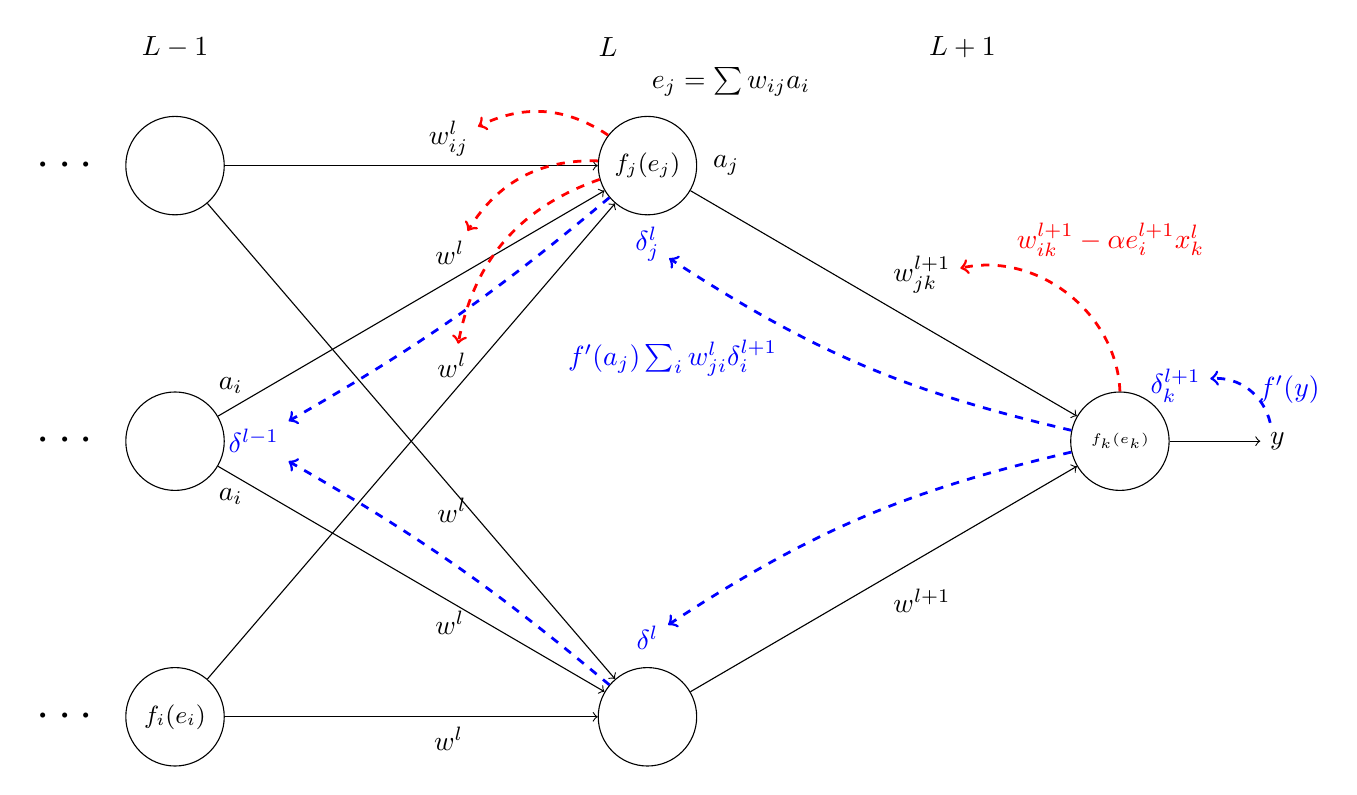
\begin{tikzpicture}

	\tikzstyle{nodo}=[circle, draw, minimum size=1.25cm]
	\tikzstyle{upw}=[dashed, red, ->, line width = 1pt]

	\coordinate (l_0) at (0, 5.0);
	\coordinate (l_1) at (5.5, 5.0);
	\coordinate (l_2) at (10, 5.0);

	\coordinate (f_1_1) at (0, 3.5); % CAPA ENTRADA
	\coordinate (f_1_2) at (0, 0); % CAPA ENTRADA
	\coordinate (f_1_3) at (0, -3.5); % CAPA ENTRADA
	\coordinate (f_2_1) at (6.0, 3.5); % CAPA OCULTA 1
	\coordinate (f_2_2) at (6.0, -3.5); % CAPA OCULTA 1
	\coordinate (f_3_1) at (12, 0); % CAPA SALIDA
	\coordinate (y) at (14, 0); % CAPA SALIDA

	\node[] (l_0) at (l_0) {$L - 1$};
	\node[] (l_1) at (l_1) {$L$};
	\node[] (l_2) at (l_2) {$L + 1$};

	\node[nodo] (f_1_1) at (f_1_1) {}; % CAPA ENTRADA
	\node[nodo] (f_1_2) at (f_1_2) {}; % CAPA ENTRADA
	\node[nodo] (f_1_3) at (f_1_3) {\small $f_i(e_i)$}; % CAPA ENTRADA
	\node[nodo] (f_2_1) at (f_2_1) {\small $f_j(e_j)$}; % CAPA OCULTA 1
	\node[nodo] (f_2_2) at (f_2_2) {}; % CAPA OCULTA 1
	\node[nodo] (f_3_1) at (f_3_1) {\tiny $f_k(e_k)$}; % CAPA SALIDA
	\node[] (y) at (y) {$y$}; % CAPA SALIDA

	\node[left of=f_1_1, node distance=1.4cm] {\LARGE $\cdots$};
	\node[left of=f_1_2, node distance=1.4cm] {\LARGE $\cdots$};
	\node[left of=f_1_3, node distance=1.4cm] {\LARGE $\cdots$};

	\draw[->] (f_1_1) -- node[pos=0.6, above] (w_1_1) {$w^{l}_{ij}$} (f_2_1);
	\draw[->] (f_1_2) -- node[pos=0.6, above] (w_1_2) {$w^{l}_{}$} (f_2_1);
	\draw[->] (f_1_3) -- node[pos=0.6, above] (w_1_3) {$w^{l}_{}$} (f_2_1);
	\draw[->] (f_1_1) node[above right of=f_1_2] {$a_{i}$} -- node[pos=0.6, below] (w_2_1) {$w^{l}_{}$} (f_2_2);
	\draw[->] (f_1_2) node[below right of=f_1_2] {$a_{i}$} -- node[pos=0.6, below] (w_2_2) {$w^{l}_{}$} (f_2_2);
	\draw[->] (f_1_3) -- node[pos=0.6, below] (w_2_3) {$w^{l}_{}$} (f_2_2);
	\draw[->] (f_2_1) node[right of=f_2_1] {$a_{j}$} -- node[pos=0.5, above right] (w_j_k) {$w^{l+1}_{jk}$} (f_3_1);
	\draw[->] (f_2_2) -- node[pos=0.5, below right] {$w^{l+1}$} (f_3_1);
	\draw[->] (f_3_1) -- node[pos=0.5, below right] {$$} (y);

	\node[above right of=f_2_1, node distance=1.5cm] {$e_{j} = \sum w_{ij}a_i$};


	\draw[upw] (f_3_1) to[bend right=50] node[above right, pos=0.8] {$w^{l+1}_{ik} - \alpha e^{l+1}_{i}x^{l}_{k}$} (w_j_k);
	\draw[upw] (f_2_1) to[bend right=30] node[above]{$$} (w_1_1);
	\draw[upw] (f_2_1) to[bend right=30] node[above]{$$} (w_1_2);
	\draw[upw] (f_2_1) to[bend right=30] node[above]{$$} (w_1_3);


	\node[blue, above right of=f_3_1] (e_i) {$\delta^{l+1}_{k}$};
	\node[blue, below of=f_2_1] (e_2_1_i) {$\delta^{l}_{j}$};
	\node[blue, above of=f_2_2] (e_2_2_i) {$\delta^{l}$};
	\node[blue, right of=f_1_2] (e_1_2_i) {$\delta^{l-1}$};

	\draw[upw, blue] (y) to[bend right=40] node[right]{$f'(y)$} (e_i);
	\draw[upw, blue] (f_3_1) to[bend left=10] node[below left, pos=0.7]{$f'(a_{j})\sum_{i}w^{l}_{ji}\delta^{l+1}_{i}$} (e_2_1_i);
	\draw[upw, blue] (f_3_1) to[bend right=10] (e_2_2_i);

	\draw[upw, blue] (f_2_1) to[bend left=5] (e_1_2_i);
	\draw[upw, blue] (f_2_2) to[bend right=5] (e_1_2_i);

\end{tikzpicture}
}
	\label{fig:vanishing}
	\caption{Gradiente descendente}
\end{imagen}

\section{Revisión de la literatura}
Muchos de los métodos utilizados \cite{Elman1990, Schmidhuber1992b, Pearlmutter1989, Pearlmutter1995} sufren del desvanecimiento del gradiente. Para solventar el problema hay diversos métodos que lo evitan.
%% 13. S. E. Fahlman, "The recurrent cascade-correlation learning algorithm", in Advances in Neural Information Processing Systems 3, ed. R. P. Lippmann et al. (Morgan Kaufmann, San Mateo, 1991), pages 190-196.

% 14. R. J. Williams, "Complexity of exact gradient computation algorithms for recurrent neural networks" , Technical Report NU-CCS-89-27, Boston: Northeastern Univ., College of Computer Science, 1989.

%% 15. J. Schmidhuber, "A fixed size storage O(n^3) time complexity learning algorithm for fully recurrent continually running networks", Neural Computation, 4(2).243-248 (1992).

%% 16. B. A. Pearlmutter, "Learning state space trajectories in recurrent neural networks", Neural Computation, 1(2):263{269 (1989).

%% 17B. A. Pearlmutter, "Gradient calculations for dynamic recurrent neural networks: A survey", IEEE Transactions on Neural Networks, 6(5):1212{1228 (1995).


\subsection{Métodos de búsqueda global}
Los métodos de búsqueda global no utilizan el gradiente. Métodos como {\em simulated annealing} (SA), {\em multi-grid random search} \cite{Bengio1994} y {\em random weight guessing} \cite{Schmidhuber1996} han sido investigados. Se ha encontrado que los métodos de búsquedas globales funcionan bien en problemas que involucren dependencias a largo plazo y que además utilizan redes que contienen pocos parámetros y no precisan de alta precisión en sus calculos.

El método SA es un algoritmo de búsqueda meta-heurística para problemas de optimización global. La técnica está basada en el proceso de calentamiento de un metal, vidrio o cristal hasta su punto de fusión, para luego enfriarlo hasta obtener una estructura cristalina. El algoritmo \ref{alg:sa} decribe el procedimiento de la siguiente manera: dada una solución inicial se genera un conjunto de soluciones que son una perturbación de la solución actual, al evaluar cada perturbación se actualizará la solución actual en caso de que la perturbación sea mejor que la solución actual, y en caso contrario, existirá una probabilidad de que la solución actual sea actualizada de igual manera.

\scalebox{0.8}{\begin{algorithm}[H]
    \SetAlgoLined
	\DontPrintSemicolon
	\KwData{Temperatura $T$, constante de Boltzmann $k$, factor de reducción $c$}
	Seleccionar el mejor vector solución $x_{0}$ a optimizar\;
	\While{El criterio no se cumpla}{
		\While{Existan soluciones en el conjunto}{
			Seleccionar una solución $x_{0} + \Delta x$\;
			\uIf{$f(x_{0} + \Delta x) < f(x_{0})$}{
				$f_{new} = f(x_{0} + \Delta x)$; $x_{0} = x_{0} + \Delta x$\;
			}
			\Else{
				$\Delta f = f(x_{0} + \Delta x) - f(x_{0})$\;
				\uIf{$rand(0, 1) > \exp{(-\Delta f/kT}$)}{
					$f_{new} = f(x_{0} + \Delta x)$; $x_{0} = x_{0} + \Delta x$\;
				}\Else{
					$f_{new} = f(x_{0})$\;
				}
			}
			$f = f_{new}$; $T = cT$\;
		}
	}
	\caption{Simulated annealing}
	\label{alg:sa}
\end{algorithm}}



% [1998b] Hochreiter
% Y. Bengio, P. Simard, and P. Frasconi, "Learning long-term dependencies with gradient descent is dicult", IEEE Transactions on Neural Networks, 5(2):157{166 (1994).
%\subsubsection{(ii) Métodos que refuerzan el gradiente}
%Los valores más grandes del gradiente pueden ser reforzados por la optimización pseudo-Newton ponderada en el tiempoy la propagación discreta del errror \cite{Bengio1994}. Presentan problemas para almacenar información real de gran valor en el tiempo.

%\subsubsection{(iii) Métodos que operan en niveles mas altos}
%Anteriormente se ha propuesto un enfoque EM para la propagación del objetivo \cite{Bengio1993}. Este enfoque utiliza un número discreto de estados y, por lo tanto, tendrá problemas con valores continuos.
%Las técnicas de filtrado de Kallman se utilizan para el entrenamiento de redes recurrentes \cite{Puskorius1994}. Sin embargo, un factor de descuento derivado conduce a problemas de desvanecimiento del gradiente.
%Si un problema de retraso a largo plazo contiene regularidades locales, un sistema jerárquico chunket funciona bien \cite{Schmidhuber1992a}.

%\subsubsection{(iv) Métodos que utilizan arquitecturas especiales}
\subsection{El modelo de memoria a corto y largo plazo}
\citeA{Hochreiter1997a} introdujeron el modelo de memoria a corto y largo plazo ({\em Long short-term memory}, LSTM) como solución al problema del devanecimiento del gradiente. La red LSTM se basa en el bloque de memoria, que se componse de una o más celdas de memoria, una compuerta de entrada y una compuerta de salida. Las entradas son unidades multiplicativas con activación continua y son compartidas por todas las celdas de un mismo bloque de memoria. Cada celda contiene una unidad lineal con una conexión recurrente local llamada carrusel de error constante (CEC), se conocerá como estado de la celda a la activación del CEC.

Cada celda recibe una entrada ponderada por los pesos correspondientes a la capa anterior. La compuerta de entrada se encarga de de permitir o impedir el acceso de estos valores al CEC del interior de la celda. La compuerta de salida realiza una acción similar sobre la salida de la celda, tolerando o reprimiendo la difusión del estado del CEC al resto de la red.

Los bloques de memoria configuran una red LSTM, donde no se indican los sesgos de las distintas neuronas del modelo. La existencia de las conexiones con pesos $W^{y, u}$  determina la naturaleza de la red. Así, si se permite la existencia de esta conexión, la red LSTM se puede considerar como una máquina neuronal de estados de MEaly, si no se permite, la red LSTM puede considerarse como una máquina nerupna de estados de Moore. El estado de la red LSTM está formado por las activaciones de las compuertas, el CEC y las celdas de los bloques de memoria.

%%%%%%%%%%%%%%%%%%%%%%%%%%%%%%%%%%%%%%%%
% LiuShenxiu.pdf
% Conquering vanishing gradient: Tensor Tree LSTM on aspect-sentiment classification
% - Tree-structures LSTMs
% - Tensor Tree LSTM


%%%%%%%%%%%%%%%%%%%%%%%%%%%%%%%%%%%%%%%%
% Lipton2015
% Truncated backpropagation through time (TBPTT) is one solution to the exploding gradient problem for continuously running networks [Williams and Zipser, 1989]


%%%%%%%%%%%%%%%%%%%%%%%%%%%%%%%%%%%%%%%%
% Squartini2003a
% PREPROCESSING BASED SOLUTION FOR THE VANISHING
% Squartini2003b
% Attempting to reduce the vanishing gradient effect through a novel recurrent multiscale architecture
\subsection{Preprocesamiento de la señal}
\citeA{Squartini2003a} propone pre-procesar la señal de entrada a través de una descomposición wavelet, buscando separar la información a corto plazo de la información a largo plazo, y entrenando diferentes NN. Los resultados son combinados para alcanzar el objetivo final. Este enfoque simplifica el proceso de aprendizaje de la NN, evitando cambios relevantes en la arquitectura de la red y las técnicas de aprendizaje.

	%\chapter{Diseño de la experimentación}
\section{Lógica del diseño}

\section{Metodología del experimento}

\section{Consideraciones generales}

	%%%%%%%%%%%%%%%%%%%%%%%%%%%%
	% Fin contenido
	%%%%%%%%%%%%%%%%%%%%%%%%%%%


	%%%%%%%%%%%%%%%%%%%%%%%%
	% Bibliografía
	%%%%%%%%%%%%%%%%%%%%%%%%
	\bibliographystyle{apacite}
	\bibliography{referencias}
	%%%%%%%%%%%%%%%%%%%%%%%%
	% Fin bibliografía
	%%%%%%%%%%%%%%%%%%%%%%%%


	%%%%%%%%%%%%%%%%%%%%%%%%
	% Apéndice
	%%%%%%%%%%%%%%%%%%%%%%%%
	% \appendix
	% \clearpage
	 %\addappheadtotoc
	% \appendixpage
	%%%%%%%%%%%%%%%%%%%%%%%%
	% Fin apéndice
	%%%%%%%%%%%%%%%%%%%%%%%%
\end{document}
